% Chapter introductions perform a similar orientation function in that they introduce the reader to the foci, 
% aims, procedure and argument of each specific chapter, and provide any other necessary reader-information for that chapter.
\chapter{Tools for data analysis}
The idea of this chapter is to show the main tools, part of Zensor's software stack, used during my work experience, in particular for performing daily data analysis task, as described in Section~\ref{section:workflow}.
This chapter is divided into three parts, each focusing on a specific pieces of software. Each developer tool covers one or more phases of the data analysis process, as explained in subsection~\ref{subsect:data_analysis_proc}:
\begin{enumerate}
    \item Data processing \& cleaning: Pandas (with Python)
    \item Data storage \& warehouse: InfluxDB
    \item Data visualization \& exploration: Grafana
\end{enumerate}
These three softwares are interesting both taken individually, as we will see shortly, and together, as we will discuss in more detail in the next chapter~\ref{chapter:use_cases}, with some practical examples.

\section{Pandas}\label{section:pandas}
Pandas is a data manipulation and analysis software library created for the Python programming language. It provides data structures and functions for manipulating numerical tables and time series. It is free software distributed under the BSD three-clause licence~\cite{Misc:OpenLDAP_license:oldap-2.7}.
The name derives from the words ``panel data'', which is an econometrics term for data sets that comprise observations for the same individuals over several time periods and, at the same time, is a parody of the term ``Python data analysis''~\cite{mckinney_data_2010}.

\subsection{Series and DataFrame}
Pandas is primarily used to analyse data. It supports data import from a variety of file formats, including comma-separated values (CSV), JSON, SQL database tables or queries, and Microsoft Excel~\cite{Misc:pandas_docs}.
Furthermore, Pandas supports a variety of data manipulation operations such as merging, reshaping, and selecting, as well as data cleaning and handling.
To accomplish these goals, Pandas defines and makes use of two important software \textit{Classes}, Series and DataFrame, which we will now briefly introduce.
\begin{figure}[ht]
    \centering
    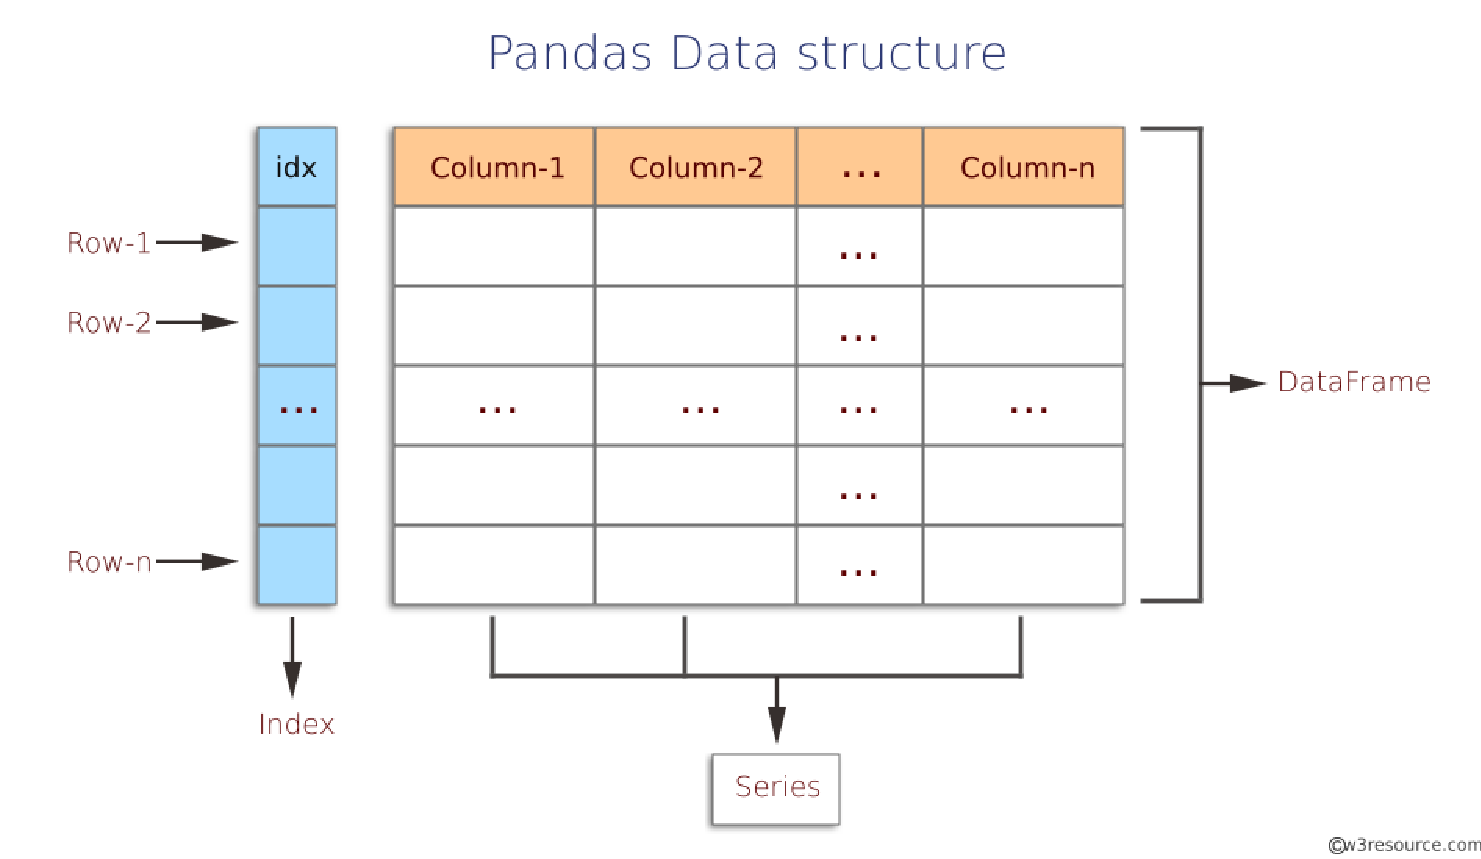
\includegraphics[width=\textwidth]{content/chapter_3/images/datastructure.pdf}
    \caption{Pandas Data structure}
    \label{fig:pandas_dataframe}
\end{figure}

\paragraph{Series} is a one-dimensional labeled array capable of holding any data type (integers, strings, floating point numbers, Python objects, etc.).
The axis labels are collectively referred to as the \textit{index}.

\paragraph{DataFrame} is a 2-dimensional labeled data structure with columns of potentially different types; in some ways it is similar to
% EB: attenzione "it's like" e` informale
a spreadsheet or an SQL table (see Figure~\ref{fig:pandas_dataframe}) in which each individual column is a \textit{Series}.
It is, generally, the most commonly used pandas object, since it accepts many different kinds of input, which makes it very flexible~\cite{reback_pandas-dev/pandas:_2022}.
% \todo{EB: controllare Inglese next ``at makes him''?? Chi?? Se \`e Pandas ``it'' non ``him''}
Along with the data, user
% one 
can optionally pass index (row labels) and columns (column labels) arguments. By doing so, the user guarantees the index and/or columns of the resulting DataFrame.
% DG: ho riformulato specificando il soggetto:
% alternativamente to secure\ to ensure per \todo{EB: ``guaranteeing the index'' non suona bene}
If axis labels are not passed, they will be constructed from the input data based on common sense rules.
And this is just one way of building a Dataframe, an appetizer of the flexibility of this library.
% \todo{EB: non so se esista ``foretaste''. Io conosco ``appetizer'' in contesti simili, ma vedi tu}

\subsection{Core Features}
The goal
% idea
of this subsection is to give an outline of how many possible use-cases are covered by this library, and, at the same time, to explore a couple of them that proved to be crucial during my internship experience.
% \todo{EB: ``Let's start'' \`e troppo informale. Meglio qualcosa come ``We are now first  illustrate ...''}
We are now first illustrate the concept of "grouping". \textit{grouping}.

\paragraph{Groupby}
The name \textbf{GroupBy} should be quite familiar to those who have used a SQL-based tool or worked with relation database. This ``engine'' allows split-apply-combine operations on heterogeneous data sets.
By ``group by'' we are referring to a process involving one or more of the following steps:
\begin{enumerate}
    \item Splitting the data into groups based on some criteria.
    \item Applying a function to each group independently.
    \item Combining the results into a data structure
\end{enumerate}
\begin{figure}[ht]
    \centering
    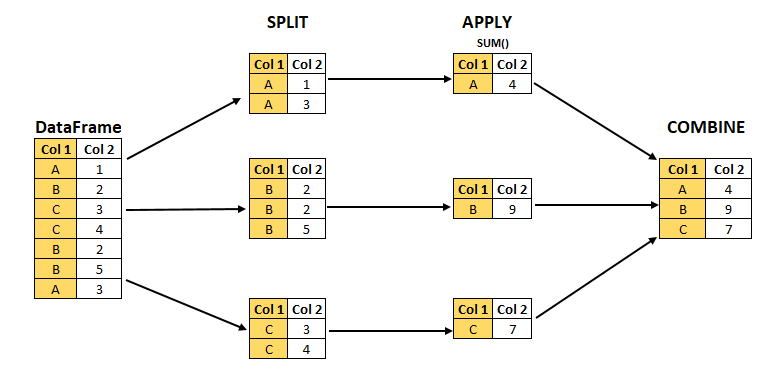
\includegraphics[width=\textwidth]{content/chapter_3/images/split-apply-combine.png}
    \caption{Shows the Split-Apply-Combine using an aggregation function (source: Analytics Vidhya~\cite{Misc:pandey_split-apply-combine})}\label{fig:pandas_groupby}
\end{figure}
Among these three steps, the \textit{split} is the most straightforward. In fact, in many situations, we would like to split the data set into groups and do something with those groups~\cite{reback_pandas-dev/pandas:_2022}.
In the \textit{apply and combine} step, we might wish to do one of the following:
\begin{itemize}
    \item Aggregation: compute a summary statistic (or statistics) for each group, some examples:
          \begin{itemize}
              \item Compute group sums or means.
              \item Compute group sizes / counts.
          \end{itemize}
    \item Transformation: perform some group-specific computations and return a like-indexed object, for instance:
          \begin{itemize}
              \item Standardize data (zscore) within a group.
              \item Filling NAs (value that are not valid) within groups with a value derived from each group.
          \end{itemize}
    \item Filtration: discard some groups, according to a group-wise computation that evaluates True or False, like:
          \begin{itemize}
              \item Discard data that belongs to groups with only a few members.
              \item Filter out data based on the group sum or mean.
          \end{itemize}
    \item Some combination of the above: \textbf{GroupBy} will examine the results of the \textit{apply} step and try to return a sensibly \textit{combined} result if it doesn't fit into either of the above two categories.
%          \todo{EB: non capisco ``sensibly'' next, DG: ho scritto la traduzione, spero sia più chiaro, se no riformulo}
\end{itemize}
Since the set of object instance methods on pandas data structures are generally rich and expressive, we often simply want to invoke, say, a DataFrame function on each group.
With this engine you can try multiple different approaches, testing what suits more your needs, even though often it is hard to define this three separate steps for badly shaped data.

\paragraph{Time series resampling}
Pandas contains extensive capabilities and features for working with time series data for all domains. Using the \textbf{NumPy} datetimes dtypes, it has consolidated a large number of features from other Python libraries (like \textbf{scikits.timeseries}) as well as created a tremendous amount of new functionality for manipulating time series data.
As an example, Pandas supports:
\begin{itemize}
    \item Parsing time series information from various sources and formats
    \item Manipulating and converting date times with timezone information
    \item Moving window statistics and linear regressions
\end{itemize}
\begin{figure}[ht]
    \centering
    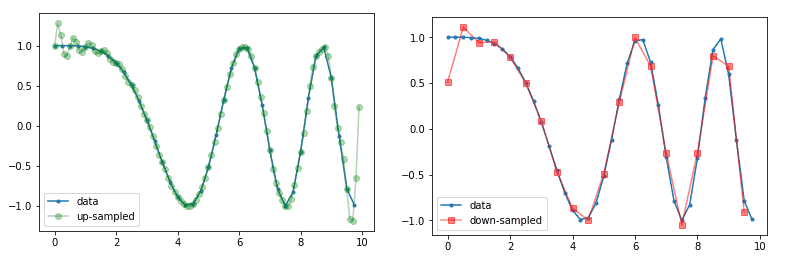
\includegraphics[width=\textwidth]{content/chapter_3/images/up-down-sample.png}
    \caption{Examples of signal waveform data processed by resample}\label{fig:up and down sampling}
\end{figure}
Let us now focus on one key aspect of handling/manipulating sensor data, crucial in our context, the necessity of resampling.
Fortunately, Pandas has, once again, a simple-to-use, powerful, and efficient functionality for performing resampling operations during frequency conversion
% \todo{EB: non sono sicuro dell'uso in Inglese di ``secondly'' e ``inutely''. Vedi un po' tu}
% l'ho preso dalla documentazione ufficiale https://pandas.pydata.org/docs/user_guide/timeseries.html#:~:text=(e.g.%2C%20converting%20secondly%20data%20into%205%2Dminutely%20data)
(e.g., converting secondly data into 5-minutely data). This is also extremely common in, but not limited to, financial applications~\cite{Misc:pandas_docs}.

To keep things simple, we could say that resample is a time-based \textbf{Groupby} followed by a reduction method on each of its groups; as a positive side,
this method can be used directly from \textit{DataFrameGroupBy} objects that we discussed in paragraph \textbf{GroupBy} previously discussed.
% \todo{EB: attenzione, i paragrafi non possono essere riferiti. Infatti, la label viene espansa con il numero della sezioine. Considerare se inserire ``il paragrafo XYZ in SectionXYZ''}
The resample function is very flexible and allows you to specify many different parameters to control the frequency conversion and resampling operation, both upsampling and downsampling.
%%%
\paragraph{Others functionality}
Furthermore, other time series features are available, and not only that notably:
\begin{itemize}
    \item Date range generation and frequency conversions
    \item Data alignment, shifting and lagging
    \item Integrated missing data handling
    \item Data set reshaping, pivoting, merging and combining
    \item Label-based slicing, sophisticated indexing, and big data set sub-setting
    \item Insertion and deletion of columns in a data structure.
\end{itemize}
\paragraph{Conlcusion}
Pandas provides a solid foundation upon which a very powerful data analysis ecosystem can be established, especially since the library is performance-optimized,
with important code paths implemented in Cython\footnote{an optimistic static Python compiler capable of using highly optimized C libraries \url{https://cython.org/}}

\section{InfluxDB}

\paragraph{Time Series} In mathematics, a time series is a series of data points which are indexed (or listed or graphed) in time order (see~\ref{fig:random time-series}). More generally, a time series is a sequence taken at evenly spaced intervals over a period of time. As a result, it's a \todo{EB: verificare ``succession''} succession of discrete-time data. Ocean tidal heights, sunspot counts, and the Dow Jones Industrial Average's daily closing value are all examples of time series.
\begin{figure}[ht]
    \centering
    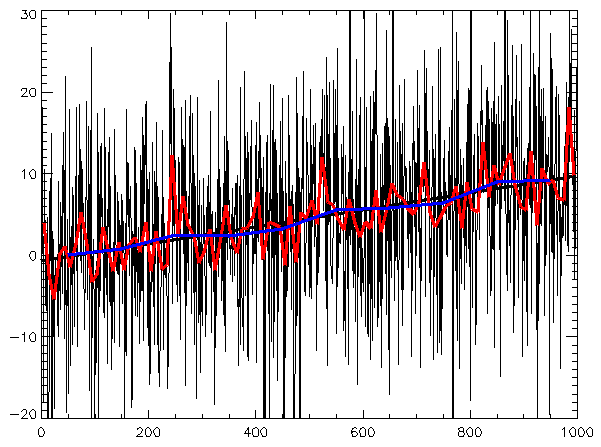
\includegraphics[width=\linewidth]{content/chapter_3/images/random-data-plus-trend-r2.png}
    \caption{Random data plus trend, with best-fit line and different smoothings applied. (source: Wikimedia Commons~\cite{file:random-data-plus-trend-r2})}
    \label{fig:random time-series}
\end{figure}
\subsection{TSDB: time series database}
It follows that a time series database \acs{tsdb} is a software system that is designed to store and serve this peculiar type of data, time series, using time(s) and value(s) pairs(s).
Timescale, popular \ac{tsdb}, CEO \textit{Ajay Kulkarni}~\cite{Misc:asay_why_time_series} put it:
\begin{quote}
    Time-series datasets track changes to the overall system as INSERTs, not UPDATEs.

    This practice of recording each and every change to the system as a new, different row is what makes time-series data so powerful. It allows us to measure change: analyse how something changed in the past, monitor how something is changing in the present, predict how it may change in the future.
    
    So here's how I like to define time-series data: data that collectively represents how a system/process/behaviour changes over time.
\end{quote}
Although it is possible to store time-series data in many diverse database types, the design of these systems with \textbf{time} as a \textbf{key} index is distinctly different from relational databases, which reduces discrete relationships through referential models.
In many cases, the repositories of time-series data will utilize compression algorithms to manage the data efficiently~\cite{Book:devops_cookbook}. Furthermore, time series databases can also be configured to regularly delete old data, unlike traditional databases which are designed to store data indefinitely.

\subsection{Influx solution}
InfluxDB is an open-source time series database \acs{tsdb} created by the InfluxData organization~\cite{Misc:influxdata_website}. It is written in the Go programming language and is used for time series data storage and retrieval in various sectors such as operations monitoring, application metrics, Internet of Things, and, especially important in our context, sensor data and real-time analytics. It also supports the processing of data from Graphite, a data logging and graphing tool for time series data. \todo{EB: ci vorrebbe forse una reference a Graphite}
\todo{Quest'ultima frase non è così rilevante}

\paragraph{Core Features}
InfluxDB has no external dependencies and provides a SQL-like vocabulary with built-in time-centric functions for querying a data structure made up of measurements, series, and points, which listens on port 8086~\cite{Misc:influx_docs}.

\begin{table}[ht]
    \centering
    \begin{tabular}{|l|l|l|l|l|}
        \hline
        time                 & location & scientist  & butterflies & honeybees \\ \hline
        2015-08-18T00:00:00Z & 1        & langstroth & 12          & 23        \\ \hline
        2015-08-18T00:00:00Z & 1        & perpetua   & 1           & 30        \\ \hline
        2015-08-18T00:06:00Z & 1        & langstroth & 11          & 28        \\ \hline
        2015-08-18T05:54:00Z & 2        & langstroth & 2           & 11        \\ \hline
        2015-08-18T06:00:00Z & 2        & langstroth & 1           & 10        \\ \hline
        2015-08-18T06:06:00Z & 2        & perpetua   & 8           & 23        \\ \hline
        2015-08-18T06:12:00Z & 2        & perpetua   & 7           & 22        \\ \hline
    \end{tabular}
    \caption{Sample time series dataset: number of butterflies and honeybees counted by two scientists}\label{tab:influx_example}
\end{table}
Each point is made up of a fieldset and a timestamp, which are key-value pairs. These pairs form a series when they are grouped together by a set of key-value pairs known as a tagset. Finally, a measurement is created by grouping series together using a string identification.
64-bit integers, 64-bit floating points, strings, and booleans are among the possible values as shown in Table~\ref{tab:influx_example}. The time and tagset are used to sort the points.
As a side note it is important to know that data is downsampled and removed according to retention policies, which are set by measurement and that \textit{Continuous Queries} are executed on a regular basis and the results are stored in a goal measurement.

\paragraph{Design Tradesoff}
InfluxDB is a time series database and \todo{EB: controllare ``optimizing''. Forse ``optimized''?} optimizing for this use case involves a number of trade-offs, primarily to increase performance at the cost of functionality~\cite{Misc:influx_docs}. Below, it is reported a list of three design ideas that lead to compromises that I personally experienced during my experience:
\begin{enumerate}
    \item Deletes are a rare occurrence. When they do occur, it is almost always against large ranges of old data that are cold for writes.
    \item Updates to existing data are a rare occurrence, and contentious updates never happen. Time series data is predominantly new data that is never updated.
    \item Many time series are ephemeral. There are often time series that appear only for a few hours and then go away, e.g., a new host that gets started and reports for a while and then gets shut down.
\end{enumerate}

\todo{Potrebbero essere più di 3, mi sembrava un buon compromesso}

\begin{table}[ht]
    \begin{tabularx}{\linewidth}{>{\parskip1ex}X@{\kern4\tabcolsep}>{\parskip1ex}X}
        \toprule
        \hfil\bfseries Pros
         &
        \hfil\bfseries Cons
        \\\cmidrule(r{3\tabcolsep}){1-1}\cmidrule(l{-\tabcolsep}){2-2}

        %% PROS, separated by empty line or \par
        Restricting access to deletes and updates allows for increased query and write performance\par
        InfluxDB is good at managing discontinuous data\par

         &

        %% CONS, separated by empty line or \par
        Delete and Update functionality is significantly restricted, since influxDB is not \acs{crud} \par
        Schema-less design means that some database functions are not supported e.g. there are no cross table joins\par
        \\\bottomrule
    \end{tabularx}
    \caption{Pros and cons of InfluxDB}
\end{table}

\paragraph{Conclusion}
It is therefore not surprising to conclude that, when compared to a general purpose relational database like SQL Server, InfluxDB, using default single node configuration, outperformed both write speed, disk storage usage (by a factor of 27x) and query execution time, where InfluxDB is up to 20x faster with an average of 8x faster~\cite{Misc:noor_2017_universit}.
It can be seen that InfluxDB, tailored-made for Time Series data, is released after the other competitive technologies (like Graphite, TimescaleDB, Prometeus) and yet still among the top list. \url{https://db-engines.com/en/ranking_trend/time+series+dbms}
\todo{Non so se valga la pena citarlo}
The InfluxQL, SQL-like query language, helps make it easier to use and adapt for people who are used to working with relational databases such as MySQL, even though influx
implementation is a smaller subset, not fully supporting \ac{crud} operations.

\section{Grafana}\label{section:grafana}
Grafana is a web-based analytics and interactive visualization application that runs on a variety of platforms.
When connected to supported data sources, it produces web-based charts, graphs, and alerts.
Grafana Enterprise, a paid version with more features, is available as a self-hosted installation or as a Grafana Labs cloud service account~\cite{Misc:grafana_labs_website}.
Grafana is split into two parts: a front end and a back end, both of which are built in TypeScript and Go.
Because the project is open source and has a large existing community, it can be expanded through a plug-in system, adding specific customizations to the existing platform~\cite{Misc:grafana_docs}.
% \todo{EB: non capisco le virgole di seguito. ``system''? DG: ora dovrebbe essere più chiaro}
Using interactive query builders, end users can develop complicated monitoring dashboards.

But what is a dashboard anyway?

\subsection{Dashboard: what is it?}
\begin{figure}[ht]
    \centering
    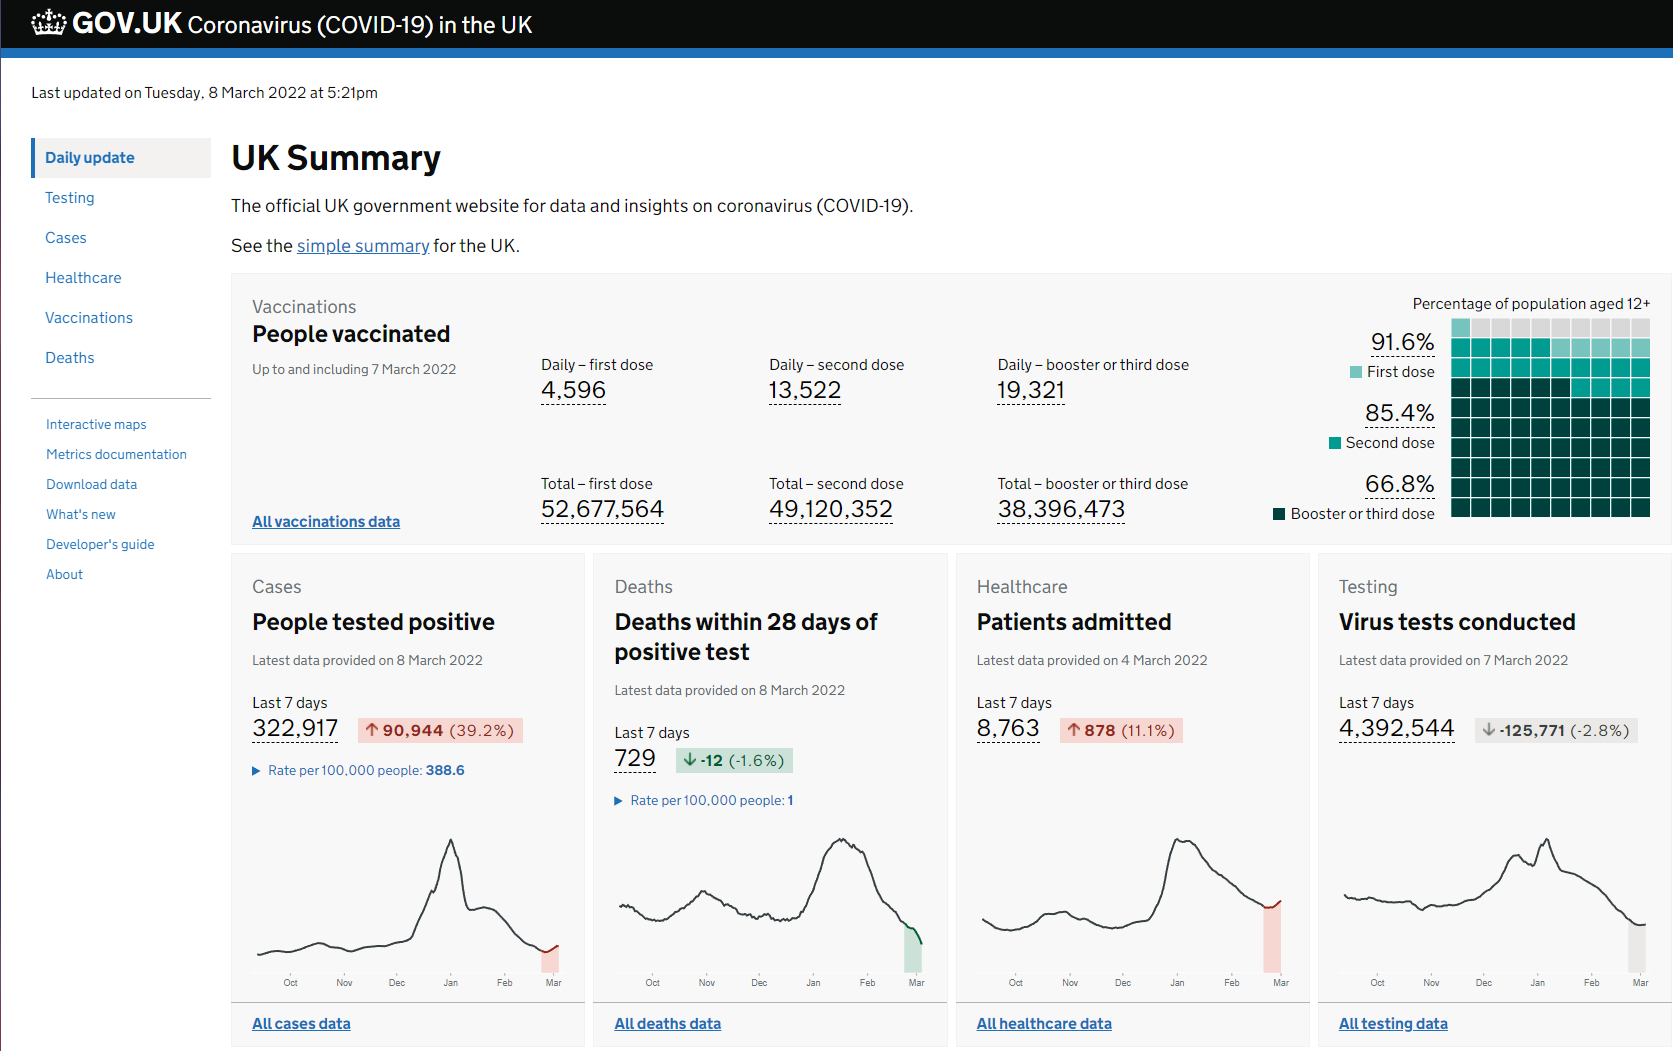
\includegraphics[width=\linewidth]{content/chapter_3/images/uk_dashboard_covid.png}
    \caption{Official data and insights on coronavirus (Source: \href{https://coronavirus.data.gov.uk/)}{gov.uk}) }
    \label{fig:corona_uk_dashboard}
\end{figure}
A dashboard, in business, is a type of graphical user interface that often enables quick access to key performance indicators (KPIs) related to a certain goal or business activity.
In our context, ``dashboard'' refers to a ``progress report'' or ``report'' and, as a type of data visualization, it is mostly accessible by a web browser and is usually linked to regularly updating data sources.
The term dashboard is derived from the automotive dashboard, where drivers may monitor the primary functions at a glance using the instrument panel.

The success of dashboard projects depends on the relevancy/importance of information provided within the dashboard. This includes the metrics chosen to monitor and the timeliness of the data forming those metrics; data must be up-to-date and accurate.
Well known dashboards include Google Analytics dashboards, used on 55\% of all websites~\cite{Misch:w3techs_usage}, which show user activity on a website, or the UK government, and similar for each country, coronavirus tracker, for the COVID-19 pandemic~\cite{Misc:uk_covid_dash}.

An interesting project is the GLAM Wiki dashboard, from Israel~\cite{Misc:wikidata_glam_project}.
Its purpose is to assist GLAM institutions (galleries, libraries, archives, and museums) in tracking the use of their free-content files that they have submitted to Wikimedia projects.
Based on multiple specified indices and several time frames, the dashboard visualizes statistical data that shows the extent of exposure and usage of these public-domain assets.
The collecting data, which is presented in a variety of diagrams and graphs, allows the institutions to obtain insights, discover patterns and preferences, and understand the overall impact of these free materials on the global audience of Wikimedia-project users.

\subsection{Key strengths}
\begin{figure}[ht]
    \centering
    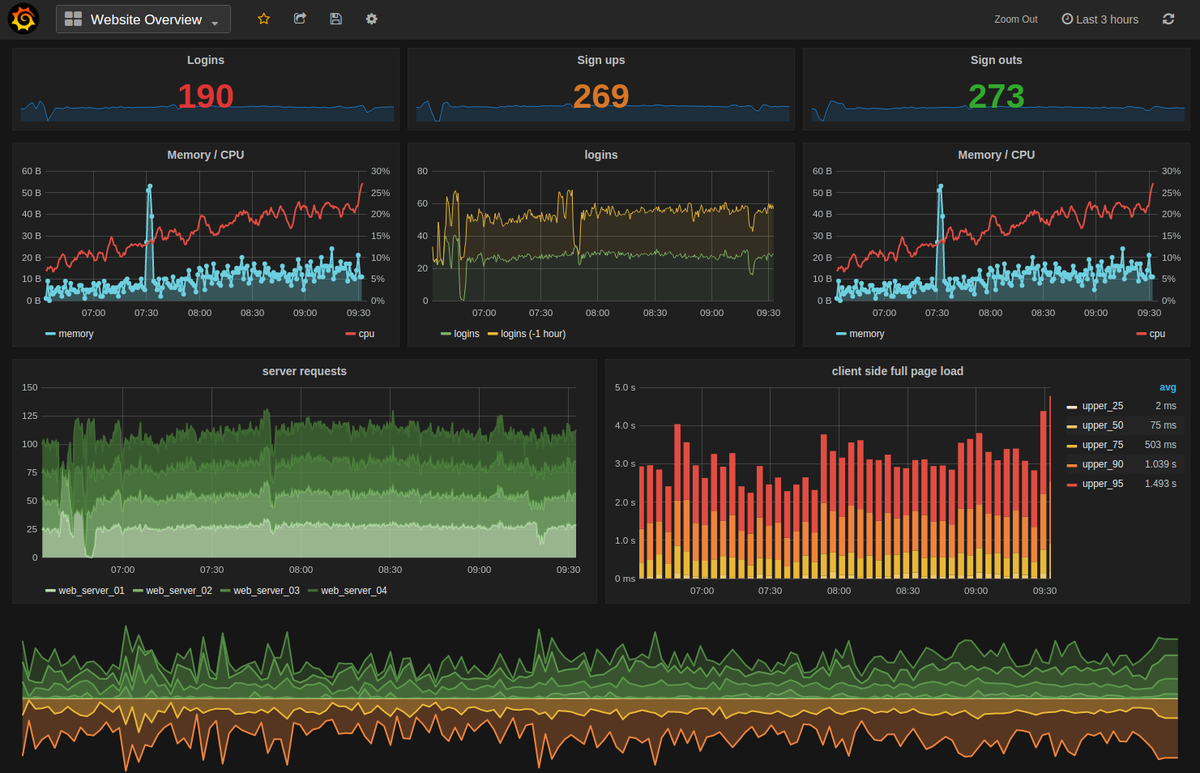
\includegraphics[width=\linewidth]{content/chapter_3/images/grafana_dashboard.png}
    \caption{Grafana Graph Visualization (Source: Flickr~\cite{file:screenshots_grafana})}
    \label{fig:grafana_dashboard}
\end{figure}
% \todo{EB: io metterei da qualche parte un altro screenshot di questo Grafana. Ma vedi te}
Now that we are familiar with the ``dashboard'' concept, we can highlight why we should use Grafana solution~\ref{fig:grafana_dashboard};
here are some of the key features~\cite{Article:comprehensive_study_grafana}:
\begin{itemize}
    \item \textbf{Visualize} fast and flexible visualization with a variety of options allows data to be displayed the way the user wants it;
    \item \textbf{Dynamic Dashboard} dynamic and reusable dashboards may be created using template variables.
    \item \textbf{Explore Metric} ad-hoc queries and dynamic drill-down permits for data discovery.
          View splits and side-by-side comparisons of different time ranges and data sources is easily achievable;
    \item \textbf{Explore Logs} fast switch from metrics to logs preserving label filters. Furthermore, searching the logs is rather quick and can be performed on live streams;
    \item \textbf{Alerting} most of the vital/operational metrics may be alerted visually and different types of notifications (SMS, mail, Slack) may be despatched with the aid of Grafana;
    \item \textbf{Mixed Data Source} the same chart can have different data source: these can be selected based on queries, with built-in support for most of the prominent data sources available in the market as well as custom ones;
    \item \textbf{Annotations} graphs may have events that can be annotated, two solutions are possible:
          use native annotation store, with the ability to add annotation events directly from the graph panel or via the HTTP API, or querying other data sources.
          Event metadata and tags can be seen when hovering over events.
\end{itemize}
\paragraph{Time ranges}
Grafana provides several ways to manage the time ranges of the data being visualized, for dashboard, panels and also for alerting,
with the support for following time units: s (seconds), m (minutes), h (hours), d (days), w (weeks), M (months), Q (quarters) and y (years).

\begin{table}[!ht]
    \centering
    \begin{tabular}{|l|l|l|}
        \toprule
        Example relative range & From:      & To:        \\ \midrule
        Last 5 minutes         & $now-5m$   & $now$      \\ \hline
        The day so far         & $now/d$    & $now$      \\ \hline
        This week              & $now/w$    & $now/w$    \\ \hline
        This week so far       & $now/w$    & $now$      \\ \hline
        This month             & $now/M$    & $now/M$    \\ \hline
        This month so far      & $now/M$    & $now$      \\ \hline
        Previous Month         & $now-1M/M$ & $now-1M/M$ \\ \hline
        This year so far       & $now/Y$    & $now$      \\ \hline
        This Year              & $now/Y$    & $now/Y$    \\ \bottomrule
    \end{tabular}
    \caption{Time units and relative ranges example}
    \label{table:time_picker}
\end{table}
The minus ($-$) operator allows you to step back in time, relative to $now$ and if the user wish to display the full period of the unit (day, week, month, etc…),
append /<time unit> to the end. It is also possible to view fiscal periods, using fQ (fiscal quarter) and fy (fiscal year) time units.
The plus ($+$) operator, instead, allows you to step forward in time relative to $now$. for example one might use this feature to look at predicted data in the future.
Here [\ref{table:time_picker}] you can see some relative ranges samples.

% \todo{EB: da qualche parte parlerei del massimo refresh rate sostenibile (se ha senso)}
The minimum dashboard refresh interval is, per default 5 seconds; this can be increased or decreased keeping in mind that
it will restrict users to set the refresh interval of a dashboard lower than given interval and anything below the default value could logically impact performance and responsiveness.

\paragraph{Loading speed}
% \texttt{And how to keep it fast}
Loading speed of a Grafana dashboard depends on 5 major things:
\begin{enumerate}
    \item  pre-selected and saved time window: the larger the queried time period, the longer it takes to open and display the contents;
    \item  data frequency in the panels: in case of the very high frequency, non aggregated data, even if selected time period is minutes, it will take time to load;
    \item  the number of panels with the data inside;
    \item  your database structure;
    \item  whether calculations have to happen inside the panel before the data is displayed.
\end{enumerate}

\paragraph{Conclusion}
Grafana is the right choice when visualizing infrastructure, applications, network devices, sensors, and more. This is a great $24/7$ monitoring solution for NOC and DevOps teams.
It can also help to manage all data from other application monitoring tools like AppDynamics, New Relic, Splunk, Dynatrace and all-in-one web interface for data viewing, alerting, and reporting.
A further comparison with other data visualization tools, such as Power BI and Tableau, might make interesting reading.

% \subsection{Operational statistics' dashboards}
% To make sure statistics page loads fast enough:

% \begin{itemize}
%     \item Take all calculations out of Grafana and only display measurement contents. Zensor Library module is available to calculate statistics on different data streams and different frequencies.
%     \item Along with the point above, make sure \textit{'time'} in the query is set to a dynamic interval and not grouped on, e.g. \textit{'1d'}
%     \item Use 'rows' to group panels together by topic and close the ones that don't have to be displayed immediately on dashboard load (and save it like that).
% \end{itemize}

% One Grafana environment allows for multiple so-called ''organizations''. 
% Every project, thus, has one ''organization'' which is visible to the client (usually named after client) 
% and another one (usually named Zensor) that is used for internal purposes.
